\documentclass[conference]{IEEEtran}
\usepackage[utf8]{inputenc}
\usepackage{amsmath,amssymb,graphicx,booktabs}

\usepackage[hidelinks,unicode,pdftitle={Averaging the Last Checkpoints of Pythia-160M: No Difference Larger Than 0.008 Nats From the Best Single Checkpoint, WikiText-2 NLL in fp32},pdfauthor={Dheiver Francisco Santos},pdfkeywords={weight averaging, checkpoint averaging, Pythia, language modeling, negative log-likelihood, numerical precision, WikiText-2},pdfsubject={Preprint, Figshare, doi:10.6084/m9.figshare.35014003}]{hyperref}
\begin{document}

\title{Averaging the Last Checkpoints of Pythia-160M: No Difference Larger Than 0.008 Nats From the Best Single Checkpoint, WikiText-2 NLL in fp32}

\author{\IEEEauthorblockN{Dheiver Francisco Santos, PhD}
\IEEEauthorblockA{Independent Researcher\\
Maceió, Alagoas, Brazil\\
ORCID: https://orcid.org/0000-0002-8599-9436\\
Preprint, Figshare, 2026, \href{https://doi.org/10.6084/m9.figshare.35014003}{doi:10.6084/m9.figshare.35014003}, CC BY 4.0}}

\maketitle

\begin{abstract}
Public intermediate checkpoints let us average a language model's own training trajectory at no training cost. We ask whether averaging the last $k$ of six Pythia-160M checkpoints (steps 143k to 100k) lowers WikiText-2 next-token negative log-likelihood (NLL) relative to the final checkpoint, and relative to the best single checkpoint. Models are evaluated in fp32. Forty validation blocks select, and 100 disjoint test blocks report. Averages with $k=2$ to $5$ lower the test NLL by $0.041$ to $0.064$ nats, with paired intervals below zero. The average at $k=6$ does not ($-0.0019$ nats). Each average also beats its own best member. However, the single 100k checkpoint already has NLL $3.5518$, $0.0616$ nats below the final one, and validation picks it. The best average ($k=5$) differs from it by $-0.0023$ nats [$-0.0083,+0.0034$]: no difference larger than $0.008$ nats detected, without an equivalence test. Pythia was trained in fp16, and an earlier bfloat16 evaluation produced a spurious $0.45$-nat gain. The evidence comes from one 160M-parameter model and one corpus.
\end{abstract}

\begin{IEEEkeywords}
weight averaging, checkpoint averaging, Pythia, language modeling, negative log-likelihood, numerical precision, WikiText-2
\end{IEEEkeywords}

\section{Introduction}
Averaging the weights of several models that share a training history is one of the cheapest interventions available for a trained network: it needs no data, no gradient steps and no extra inference cost. For a model released with intermediate checkpoints, the candidates are already on disk. The practical question for a practitioner who holds a handful of late checkpoints is concrete: does averaging the last $k$ of them lower held-out NLL, and does it beat simply picking the best single checkpoint?

This paper answers that question for one model, Pythia-160M \cite{biderman2023pythia}, using six public checkpoints from step 100k to the final step 143k, and one language-modeling corpus, WikiText-2 \cite{merity2016pointer}. We wrote down the question, the grid $k\in\{1,\dots,6\}$, the metric and the success criterion before evaluating any averaged model. A validation set of text blocks selects among candidates. The reported numbers come from a disjoint test set.

The contribution is a measurement, not a method: (i) a paired, block-level estimate of how much averaging lowers NLL relative to the final checkpoint; (ii) the observation that the best average ($k=5$) is not distinguishable from the best single checkpoint of the whole grid (step 100k, at the edge of the grid), so averaging adds nothing measurable over choosing well there, although every average beats its own best member; and (iii) a precision warning. A previous version of this manuscript reported a $0.45$-nat gain from bfloat16 evaluation. That gain was an artifact, and all numbers here are fp32.

\section{Related Work}
\textbf{Weight averaging along a trajectory.} Stochastic weight averaging (SWA) averages iterates collected along the tail of SGD and reports flatter optima and better generalization in image classification \cite{izmailov2018swa}. For language-model pre-training, Sanyal et al.\ average checkpoints of models they pretrained (nanoGPT-2, 125M--770M parameters) and also report results for public Pythia checkpoints from 1B to 12B \cite{sanyal2023lawa}. Liu et al.\ merge checkpoints of their own pre-training runs, with weights found by Bayesian optimization \cite{liu2024ckptmerge}.

\textbf{Public checkpoints.} Pythia releases intermediate training checkpoints for a model suite \cite{biderman2023pythia}, which lets anyone average points of a known trajectory without retraining. We use this resource.

\textbf{Why averaging can work, and when it may fail.} Two models can be averaged without a barrier in loss when they are linearly mode connected, a property that depends on shared early training \cite{frankle2019lmc}. Averaging fine-tuned models from a common initialization improves accuracy in the model-soups setting, which also relates weight averaging to ensembling of logits \cite{wortsman2022soups}. Weight-space arithmetic is used to edit models \cite{ilharco2022taskarith}, and Fisher-weighted averaging weights parameters by importance \cite{matena2021fisher}. Permutation symmetries have been proposed as an obstacle to averaging independently trained networks, which alignment can partly remove \cite{ainsworth2022rebasin}; this is not an issue for checkpoints of one run. Surveys of model merging cover these methods \cite{yang2024mergingsurvey,li2023fusionsurvey}, a large-scale study examines merging at scale \cite{yadav2024scale}, and a toolkit implements the averaging used here \cite{goddard2024mergekit}.

\textbf{Statistics of evaluation.} Reporting paired differences with intervals, rather than single numbers, is recommended for language-model evaluation \cite{miller2024errorbars}, and adaptive reuse of the same data for choosing and reporting can invalidate statistical estimates \cite{dwork2014adaptive}. The bootstrap supplies the intervals \cite{efron1979bootstrap}.

\textbf{Gap.} We do not know of a split-disciplined, paired block-level measurement at Pythia-160M that compares checkpoint averages with the best single checkpoint. This paper reports one for one model and one corpus.

\textbf{Author's related work.} The author's technical notes cover neighboring topics in language-model training: model merging for capability composition \cite{santos2026modelmergingfo}, curriculum learning and data-efficient pretraining \cite{santos2026curriculumlear}, knowledge distillation and self-distillation \cite{santos2026knowledgedisti}, parameter-efficient fine-tuning (LoRA, QLoRA, DoRA) \cite{santos2026parametereffic}, mixture-of-experts training and sparse upcycling \cite{santos2026mixtureofexper}, and synthetic data generation and self-improvement \cite{santos2026syntheticdatag}. This paper instead reports a controlled held-out measurement. In a different domain, the author's JEPA preprint \cite{santos2026collapseresist} uses a similar controlled-comparison style (identical budgets, several seeds, confidence intervals).

\section{Method}
Let $\theta_s$ denote the weights of the Pythia-160M checkpoint at training step $s$. The checkpoints, ordered from last to farthest, are
$S=(s_1,\dots,s_6)=(143\mathrm{k},140\mathrm{k},130\mathrm{k},120\mathrm{k},110\mathrm{k},100\mathrm{k})$. For $k\in\{1,\dots,6\}$ the averaged model is
\begin{equation}
\bar\theta_k=\frac{1}{k}\sum_{j=1}^{k}\theta_{s_j},
\end{equation}
with equal weights, computed in fp32 and used without rounding. The case $k=1$ is the unmodified final checkpoint.

\subsection*{Equations and their meaning}
Eq.~(1) is the plain mean of the first $k$ checkpoints in the list: $k=1$ is the last checkpoint, $k=2$ adds step 140k, and so on down to step 100k at $k=6$. Adding checkpoints also widens the span of steps averaged ($0$, $3$k, $13$k, $23$k, $33$k, $43$k steps back), so $k$ and the distance of the farthest checkpoint change together.

For a text block $b$ of $L=512$ consecutive tokens $x_1,\dots,x_{L+1}$, the per-block NLL of a model with weights $\theta$ is
\begin{equation}
\ell_b(\theta)=-\frac{1}{L}\sum_{i=1}^{L}\log p_\theta(x_{i+1}\mid x_{\le i}),
\end{equation}
the mean cross-entropy in nats per token of predicting each next token from its prefix inside the block. Lower is better; $e^{\ell}$ is the corresponding perplexity.

The quantity of interest is the paired NLL change over the test blocks $\mathcal{B}$,
\begin{equation}
\Delta(\theta,\theta')=\frac{1}{|\mathcal{B}|}\sum_{b\in\mathcal{B}}\big[\ell_b(\theta)-\ell_b(\theta')\big],
\end{equation}
which is negative when $\theta$ has lower NLL than the reference $\theta'$. We use $\theta'=\bar\theta_1$ (the last checkpoint) and $\theta'=$ the best single checkpoint. Pairing removes the large block-to-block variation in difficulty. The interval is the 2.5--97.5 percentile of $5000$ bootstrap resamples of blocks with replacement; the two-sided $p$ is the bootstrap tail share, and $p=0.000$ means that no resample crossed zero.

\section{Experimental Protocol}
\textbf{Models.} Pythia-160M (EleutherAI, Apache-2.0) \cite{biderman2023pythia} at revisions \texttt{step143000}, \texttt{step140000}, \texttt{step130000}, \texttt{step120000}, \texttt{step110000} and \texttt{step100000}; Hub commit hashes are in Data and Code Availability. Models are evaluated in float32 on Apple Silicon (MPS), PyTorch 2.8.0, transformers 4.57.6, with the same perplexity code for singles and averages; averaged weights are not rounded. No training is performed and the evaluation is deterministic, so there are no random seeds; the only randomness is the bootstrap (seed 0).

\textbf{Data and splits.} The corpus is the WikiText-2 test text (\texttt{wikitext-2-raw-v1}) \cite{merity2016pointer}, joined with blank lines, tokenized with the Pythia tokenizer, and cut into consecutive blocks of 512 tokens (513 tokens per block, 512 predicted). Block indices $0$--$39$ form the validation set (40 blocks) and indices $40$--$139$ the test set (100 blocks), so the two sets are disjoint but adjacent stretches of the same document collection. All 140 blocks are scored with no context carried between blocks.

\textbf{Hypothesis and selection.} The pre-registered hypothesis (written before any averaging) is that averaging the last $k=2,\dots,6$ checkpoints reduces NLL relative to the last checkpoint. The success criterion is a 95\% paired CI of the NLL change with upper limit below zero. The candidate set has 12 members: the six single checkpoints and the five averages $k=2,\dots,6$. The candidate with the lowest mean validation NLL is selected; the test set is used only to report.

\textbf{Baselines.} The pre-registered baseline is the best original (single) checkpoint by validation NLL. All six singles were evaluated on the same blocks. The last checkpoint (143k) is a second reference, because it is what a practitioner gets by default.

\textbf{Statistics.} Block-level paired bootstrap, 5000 resamples, seed 0, 95\% percentile intervals (shown as $[\text{lower},\text{upper}]$ in nats per token). The bootstrap uses $B=5{,}000$ resamples as pre-registered (\texttt{experiments/PREREG.md}); there is no deviation. The 40/100 validation/test split, the 12-candidate set and the fp32 evaluation were not in the pre-registration; fp32 is a later correction, declared above. Blocks are consecutive text and are not independent draws from the corpus, so the intervals describe variation across these 100 blocks and may understate the uncertainty about other text. No multiplicity correction is applied, and no claim relies on a nominal $p$ near a threshold.

\section{Results}
Table~\ref{tab:avg} gives validation and test NLL for the six single checkpoints and the averages, with paired differences to the last checkpoint. Fig.~\ref{fig:avg} plots the same quantities.

\begin{table*}[!t]
\caption{WikiText-2 NLL (nats per token), fp32, of single Pythia-160M checkpoints and of averages of the last $k$ checkpoints. Validation: 40 blocks; test: 100 blocks. $\Delta$ is the paired test difference to the last checkpoint (143k) with 95\% bootstrap CI over blocks. Source: \texttt{results/summary\_art07\_fp32.txt}.}
\label{tab:avg}
\centering
\small
\begin{tabular}{llccr}
\toprule
Type & Checkpoint(s) & Val NLL & Test NLL & $\Delta$ vs.\ 143k [95\% CI] \\
\midrule
single & 143k (last) & 3.6614 & 3.6134 & --- \\
single & 140k & 3.6362 & 3.5933 & $-0.0201$ [$-0.0252$, $-0.0150$] \\
single & 130k & 3.6300 & 3.5933 & $-0.0201$ [$-0.0256$, $-0.0141$] \\
single & 120k & 3.6287 & 3.5966 & $-0.0167$ [$-0.0218$, $-0.0117$] \\
single & 110k & 3.5895 & 3.5580 & $-0.0554$ [$-0.0606$, $-0.0502$] \\
single & 100k & 3.5832 & 3.5518 & $-0.0616$ [$-0.0678$, $-0.0551$] \\
\midrule
avg $k=2$ & 143k, 140k & 3.6195 & 3.5728 & $-0.0406$ [$-0.0433$, $-0.0378$] \\
avg $k=3$ & 143k--130k & 3.6012 & 3.5591 & $-0.0543$ [$-0.0574$, $-0.0511$] \\
avg $k=4$ & 143k--120k & 3.5959 & 3.5552 & $-0.0582$ [$-0.0617$, $-0.0547$] \\
avg $k=5$ & 143k--110k & 3.5872 & 3.5495 & $-0.0639$ [$-0.0677$, $-0.0602$] \\
avg $k=6$ & 143k--100k & 3.6473 & 3.6115 & $-0.0019$ [$-0.0071$, $+0.0034$] \\
\bottomrule
\end{tabular}
\end{table*}

\begin{figure}[!t]
\centering
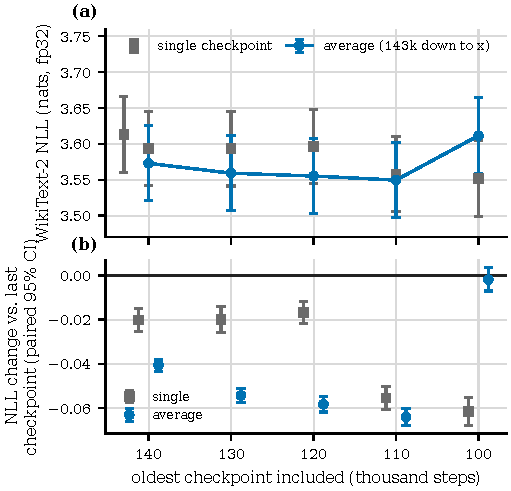
\includegraphics[width=\columnwidth]{figs/fig07_pythia_avg.pdf}
\caption{Pythia-160M on WikiText-2 in fp32. (a) NLL of each single checkpoint and of each average of the last $k$ checkpoints. Panel (a) error bars are $\pm1.96$ unpaired standard errors over blocks. (b) Paired test-NLL difference relative to the last checkpoint (143k), with 95\% bootstrap CI over blocks (paired).}
\label{fig:avg}
\end{figure}

\textbf{Pre-registered hypothesis.} Supported against the last checkpoint for $k=2,\dots,5$: the paired intervals lie entirely below zero, with changes of $-0.041$, $-0.054$, $-0.058$ and $-0.064$ nats (bootstrap $p=0.000$ in all four). It is not supported for $k=6$: $-0.0019$ nats [$-0.0071$, $+0.0034$], $p=0.459$. In perplexity units (exp of mean NLL) the last checkpoint scores $37.1$ and the $k=5$ average $34.8$.

\textbf{The best single checkpoint versus the best average.} The single 100k checkpoint has test NLL $3.5518$, which is $0.0616$ nats [$-0.0678$, $-0.0551$] below the last checkpoint and gives perplexity $34.9$. It also has the lowest validation NLL of the six singles, so it is the pre-registered baseline. The best average on validation is $k=5$. Its test difference to the 100k single is $-0.0023$ nats [$-0.0083$, $+0.0034$], $p=0.417$: no difference larger than $0.008$ nats detected; there is no equivalence test and no margin was set. Among the 12 candidates, validation selects the single 100k checkpoint, whose gain over the last checkpoint on test is $-0.0616$ nats [$-0.0678$, $-0.0551$]. Most of the gain of averaging over the last checkpoint is therefore available by choosing an earlier checkpoint. The averages are not merely their worst parts, though: each average beats the best single checkpoint among its own members (descriptive, test set). For $k=2$, $3$ and $4$ the best member is 140k, and the differences are $-0.0205$ [$-0.0234$, $-0.0176$], $-0.0342$ [$-0.0376$, $-0.0308$] and $-0.0381$ [$-0.0415$, $-0.0347$]. For $k=5$ the best member is 110k, and the difference is $-0.0085$ [$-0.0123$, $-0.0048$]. What no average does is beat the 100k single, which enters the average only at $k=6$. (Source: \texttt{results/summary\_art07\_fp32.txt}, lines ``melhor membro''.)

\textbf{Non-monotone trajectory.} On WikiText-2 the later checkpoints of Pythia-160M have higher NLL than earlier ones: 143k is worse than 110k and 100k, and the single-checkpoint test NLL falls from $3.6134$ at 143k to $3.5518$ at 100k. We did not test the cause. Possible causes are a shift between the training distribution and WikiText-2 over training, or the final decay of the learning rate. Both are conjectures. The average at $k=6$ is worse than $k=5$ ($3.6115$ versus $3.5495$ test NLL) although it adds the best single checkpoint; averaging the farthest checkpoint with the last five does not help here, and we do not know why.

\textbf{What the result does not show.} It does not show that averaging beats the best single checkpoint of the grid, nor that it is worse; the interval allows differences of about $0.008$ nats in favor of the average and $0.003$ against it, and there is no equivalence test. It does not show the effect for other model sizes, other Pythia checkpoints, other corpora or downstream accuracy. The grid ends at step 100k, so checkpoints older than 100k were not tested.

\subsection*{Evaluation precision}
Pythia was trained in fp16. Evaluating the same checkpoints in bfloat16 changes the numbers by about one nat (Table~\ref{tab:prec}). The last checkpoint scores $4.6074$ in bfloat16 and $3.6134$ in fp32. In bfloat16, $k=6$ appears to cut the NLL from $4.6074$ to $4.1583$ ($-0.45$ nats); in fp32 the same change is $-0.0019$ nats and not distinguishable from zero. The previous version of this manuscript reported the bfloat16 numbers. That large gain was a precision artifact, and it is corrected here. The practical rule is to check fp32 before trusting any gain on models trained in fp16.

\begin{table}[!t]
\caption{Test NLL of the average of the last $k$ checkpoints in bfloat16 and fp32 (100 test blocks). Source: \texttt{results/summary\_art07\_fp32.txt}.}
\label{tab:prec}
\centering
\small
\begin{tabular}{cccc}
\toprule
$k$ & bf16 & fp32 & bf16 $-$ fp32 \\
\midrule
1 & 4.6074 & 3.6134 & $+0.9940$ \\
2 & 4.5483 & 3.5728 & $+0.9755$ \\
3 & 4.5082 & 3.5591 & $+0.9490$ \\
4 & 4.4810 & 3.5552 & $+0.9258$ \\
5 & 4.4412 & 3.5495 & $+0.8917$ \\
6 & 4.1583 & 3.6115 & $+0.5468$ \\
\bottomrule
\end{tabular}
\end{table}

\section{Discussion and Limitations}
\textbf{A plausible explanation, not tested.} A common intuition, which we did not test, is that averaging reduces the noise that stochastic gradient steps leave in the weights. Here it would explain why averages of $k=2$ to $5$ beat the last checkpoint. It does not explain why they do not beat the single 100k checkpoint, which they only approach. We measured no gradient noise, sharpness, learning-rate state or loss along the line between checkpoints.

\textbf{Threats to validity.} (i) Grid boundary: the farthest checkpoint is 100k, and it is also the best single one, so better checkpoints may lie earlier in training. (ii) Scale and scope: a single 160M-parameter model, one training trajectory, one corpus and one metric (NLL); no downstream benchmark was run. (iii) Block structure: the 140 blocks are consecutive stretches of one corpus, and validation and test are adjacent rather than randomly interleaved. Blocks are not independent, so the intervals reflect variation across these blocks only. (iv) Precision: evaluation is in fp32 and the previous bfloat16 result was an artifact; we did not test fp16 or other precisions. (v) We did not check for contamination of WikiText-2 in the pre-training corpus. It would affect all checkpoints and not the paired difference, but it could affect which checkpoints look good on this text. (vi) The comparison is on NLL only; a lower WikiText-2 NLL does not imply better generation or task accuracy.

\textbf{Use.} For a practitioner with these six public checkpoints and an NLL objective on WikiText-2, averaging the last five beats the default last checkpoint and beats its own best member, but is not distinguishable from the best single checkpoint of the whole grid (100k, at the grid edge), which needs no averaging. Choose a checkpoint on held-out data first; relative to that best single checkpoint, averaging is not needed here.

\section{Conclusion}
On the Pythia-160M trajectory from step 100k to 143k, averaging the last $k=2$ to $5$ checkpoints lowers fp32 WikiText-2 NLL relative to the final checkpoint by $0.041$ to $0.064$ nats, with paired block-level intervals below zero, while $k=6$ does not. Each average also beats its own best member. But the single 100k checkpoint is better than the final one by $0.0616$ nats, validation selects it, and the best average is not distinguishable from it ($-0.0023$ nats, CI $[-0.0083,+0.0034]$; no difference larger than $0.008$ nats detected, no equivalence test). A bfloat16 evaluation, reported in an earlier version, showed a spurious $0.45$-nat gain; models trained in fp16 should be checked in fp32. The result comes from one model and one corpus, and the cause of the late-checkpoint degradation is untested.

\section*{Data and Code Availability}
All code, per-block results and summaries are in the repository \texttt{artigos-pesos-modelos-pequenos} at git tag \texttt{preprints-v1} (the commit that contains this manuscript and all scripts and caches); the pre-registration is \texttt{experiments/PREREG.md} (written before any averaging). The numbers in this paper come from \texttt{results/summary\_art07\_fp32.txt}, produced by \texttt{experiments/an\_art07\_fp32.py} from the cached per-block fp32 NLL (\texttt{cache/fp32\_p\_single*.npz}, \texttt{cache/fp32\_p\_avg*.npz}, computed by \texttt{experiments/fp32\_check.py}); the bfloat16 comparison uses \texttt{cache/p\_avg*\_\_ppl40\_100.npz}. One command regenerates tables and figure: \texttt{./run\_everything.sh}. Versions: Python 3.9.6, PyTorch 2.8.0, transformers 4.57.6, numpy 1.26.4, datasets 4.5.0. Pythia-160M Hub revisions (commit): step143000 \texttt{b56d9bee}, step140000 \texttt{d846b982}, step130000 \texttt{0b59d075}, step120000 \texttt{3df7d2c5}, step110000 \texttt{8dbf3af7}, step100000 \texttt{c507d0e6} (full hashes in \texttt{MANIFEST.json}). WikiText-2 is \texttt{Salesforce/wikitext}, config \texttt{wikitext-2-raw-v1}. The evaluation is deterministic; the bootstrap seed is 0.

\section*{Acknowledgments}
No external funding.

\begin{thebibliography}{99}
\bibitem{biderman2023pythia} S. Biderman, H. Schoelkopf, Q. Anthony, et al., ``Pythia: A suite for analyzing large language models across training and scaling,'' in \emph{Proc.\ ICML}, 2023, arXiv:2304.01373.
\bibitem{merity2016pointer} S. Merity, C. Xiong, J. Bradbury, and R. Socher, ``Pointer sentinel mixture models,'' in \emph{Proc.\ ICLR}, 2017, arXiv:1609.07843.
\bibitem{izmailov2018swa} P. Izmailov, D. Podoprikhin, T. Garipov, D. Vetrov, and A. G. Wilson, ``Averaging weights leads to wider optima and better generalization,'' in \emph{Proc.\ UAI}, 2018, arXiv:1803.05407.
\bibitem{sanyal2023lawa} S. Sanyal, A. Neerkaje, J. Kaddour, et al., ``Early weight averaging meets high learning rates for LLM pre-training,'' arXiv:2306.03241, 2023.
\bibitem{liu2024ckptmerge} D. Liu, Z. Wang, B. Wang, et al., ``Checkpoint merging via Bayesian optimization in LLM pretraining,'' arXiv:2403.19390, 2024.
\bibitem{frankle2019lmc} J. Frankle, G. K. Dziugaite, D. M. Roy, and M. Carbin, ``Linear mode connectivity and the lottery ticket hypothesis,'' in \emph{Proc.\ ICML}, 2020, arXiv:1912.05671.
\bibitem{wortsman2022soups} M. Wortsman, G. Ilharco, S. Y. Gadre, et al., ``Model soups: Averaging weights of multiple fine-tuned models improves accuracy without increasing inference time,'' in \emph{Proc.\ ICML}, 2022, arXiv:2203.05482.
\bibitem{matena2021fisher} M. Matena and C. Raffel, ``Merging models with Fisher-weighted averaging,'' in \emph{Proc.\ NeurIPS}, 2022, arXiv:2111.09832.
\bibitem{ainsworth2022rebasin} S. K. Ainsworth, J. Hayase, and S. Srinivasa, ``Git Re-Basin: Merging models modulo permutation symmetries,'' in \emph{Proc.\ ICLR}, 2023, arXiv:2209.04836.
\bibitem{yang2024mergingsurvey} E. Yang, L. Shen, G. Guo, et al., ``Model merging in LLMs, MLLMs, and beyond: Methods, theories, applications and opportunities,'' arXiv:2408.07666, 2024.
\bibitem{li2023fusionsurvey} W. Li, Y. Peng, M. Zhang, et al., ``Deep model fusion: A survey,'' arXiv:2309.15698, 2023.
\bibitem{yadav2024scale} P. Yadav, T. Vu, J. Lai, et al., ``What matters for model merging at scale?'' arXiv:2410.03617, 2024.
\bibitem{goddard2024mergekit} C. Goddard, S. Siriwardhana, M. Ehghaghi, et al., ``Arcee's MergeKit: A toolkit for merging large language models,'' in \emph{Proc.\ EMNLP Industry Track}, 2024, arXiv:2403.13257.
\bibitem{miller2024errorbars} E. Miller, ``Adding error bars to evals: A statistical approach to language model evaluations,'' arXiv:2411.00640, 2024.
\bibitem{dwork2014adaptive} C. Dwork, V. Feldman, M. Hardt, T. Pitassi, et al., ``Preserving statistical validity in adaptive data analysis,'' in \emph{Proc.\ STOC}, 2015, arXiv:1411.2664.
\bibitem{efron1979bootstrap} B. Efron, ``Bootstrap methods: Another look at the jackknife,'' \emph{Ann.\ Statist.}, vol.~7, no.~1, pp.~1--26, 1979, doi:10.1214/aos/1176344552.
\bibitem{ilharco2022taskarith} G. Ilharco, M. T. Ribeiro, M. Wortsman, et al., ``Editing models with task arithmetic,'' in \emph{Proc.\ ICLR}, 2023, arXiv:2212.04089.
\bibitem{santos2026modelmergingfo} D. F. Santos, ``Model Merging for Capability Composition: A Technical Note,'' Zenodo, 2026, doi:10.5281/zenodo.21610555.
\bibitem{santos2026collapseresist} D. F. Santos, ``Collapse-Resistant Joint-Embedding Predictive Architectures: A Controlled Comparison of SIGReg, VICReg, and EMA,'' Zenodo, v2, 2026, doi:10.5281/zenodo.24223364.
\bibitem{santos2026curriculumlear} D. F. Santos, ``Curriculum Learning and Data-Efficient Pretraining: A Technical Note,'' Zenodo, 2026, doi:10.5281/zenodo.21610595.
\bibitem{santos2026knowledgedisti} D. F. Santos, ``Knowledge Distillation and Self-Distillation for Language Models,'' Zenodo, 2026, doi:10.5281/zenodo.21610100.
\bibitem{santos2026parametereffic} D. F. Santos, ``Parameter-Efficient Fine-Tuning: LoRA, QLoRA, and DoRA,'' Zenodo, 2026, doi:10.5281/zenodo.21610033.
\bibitem{santos2026mixtureofexper} D. F. Santos, ``Mixture-of-Experts Training and Sparse Upcycling,'' Zenodo, 2026, doi:10.5281/zenodo.21610062.
\bibitem{santos2026syntheticdatag} D. F. Santos, ``Synthetic Data Generation and Self-Improvement: A Technical Note,'' Zenodo, 2026, doi:10.5281/zenodo.21610525.
\end{thebibliography}

\end{document}
